% Note: This file intended to be included in one of the two wrapper files in this directory.
% Hence, it has no document class.

\usepackage[utf8]{inputenc}
\usepackage{minted}
\usepackage{listings}
\usepackage{graphicx}
\usepackage{xcolor}
\usepackage{adjustbox}


\usetheme{Madrid}
\useinnertheme{circles}
\definecolor{ssgreen}{HTML}{669B41}
\usecolortheme[named=ssgreen]{structure}
\setbeamertemplate{navigation symbols}{}
\setlength{\columnseprule}{0.4pt}

\AtBeginEnvironment{frame}{\setcounter{footnote}{0}}

\title[Kubernetes]{Introduction to Kubernetes}
\author[Ed MacDonald]{Ed MacDonald\\emacdonald@solutionstreet.com}
\institute[\href{https://solutionstreet.com}{SolutionStreet}]{SolutionStreet\\\href{https://solutionstreet.com}{(solutionstreet.com)}}
\date{October 2020}

\titlegraphic{ \includegraphics[width=2cm]{logo} }

\begin{document}
    \frame{\titlepage}
    \begin{frame}
        \frametitle{Solution Street is Hiring\footnotemark}
        \begin{minipage}[t]{0.45\textwidth}
            \vspace{0pt}
            \begin{block}{About Us}
                \begin{itemize}
                    \item{Software engineering firm founded in 2002 \textbf{by} a software engineer \textbf{for} software engineers.}
                    \item{We develop lasting relationships with our clients and retain a team of great engineers who love what they do.}
                \end{itemize}
            \end{block}
        \end{minipage}%
        \hfill
        \begin{minipage}[t]{0.45\textwidth}
            \vspace{0pt}
            \begin{block}{Immediate Need for}
                \begin{itemize}
                    \item{Senior Java Developers}
                    \item{Senior Ruby Developers}
                    \item{Senior Python Developers}
                    \item{Senior .NET Developers}
                \end{itemize}
            \end{block}
        \end{minipage}
        \footnotetext[1]{\href{https://www.solutionstreet.com/join.php}{https://www.solutionstreet.com/join.php}}
    \end{frame}

    \begin{frame}
        \frametitle{What is Kubernetes?}
        \begin{itemize}
            \item{A Container Orchestration Framework.}\pause
            \item{Very well suited for Applications that scale horizontally (stateless).}\pause
            \item{But can also accommodate portions of your infrastructure that do not scale horizontally (stateful). Don't let people tell you otherwise.}
        \end{itemize}
    \end{frame}

    \begin{frame}
        \frametitle{How do you use it?}
        \begin{itemize}
            \item{Package your Application components as Containers.}\pause
            \item{Run the Containers on Kubernetes Pods.}\pause
            \item{Let Kubernetes manage the Pods for you!}
        \end{itemize}
    \end{frame}

    \begin{frame}
        \frametitle{Why go through the hassle? (It can be a hassle)}
        Kubernetes can manage resources for you by:\pause
        \begin{itemize}
            \item{Changing the number of running Pods to meet traffic demands.}\pause
            \item{Adjusting compute resources to meet compute demands.}\pause
            \item{Replacing unresponsive Pods with new ones.}
        \end{itemize}
    \end{frame}

    \begin{frame}
        \begin{center}
            \Huge High Level Deployment Walkthrough
        \end{center}
    \end{frame}

    \begin{frame}
        \frametitle{Deploying An App: Build Your App}
        \includegraphics[width=\textwidth,height=0.85\textheight,keepaspectratio]{graphics/deploy-00-app.eps}
    \end{frame}

    \begin{frame}
        \frametitle{Deploying An App: Package Your App as a Container}
        \includegraphics[width=\textwidth,height=0.85\textheight,keepaspectratio]{graphics/deploy-01-appContainerized.eps}
    \end{frame}

    \begin{frame}
        \frametitle{Deploying An App: Push The Container to a Repository}
        \includegraphics[width=\textwidth,height=0.85\textheight,keepaspectratio]{graphics/deploy-02-containerToRepo.eps}
    \end{frame}

    \begin{frame}
        \frametitle{Deploying An App: Deploy Pods to a Kubernetes Cluster}
        \includegraphics[width=\textwidth,height=0.85\textheight,keepaspectratio]{graphics/deploy-03-emptyPods.eps}
    \end{frame}

    \begin{frame}
        \frametitle{Deploying An App: Pods Pull Your Container}
        \includegraphics[width=\textwidth,height=0.85\textheight,keepaspectratio]{graphics/deploy-04-podsWithContainers.eps}
    \end{frame}

    \begin{frame}
        \begin{center}
            \Huge Simple, right? Now let's get into the weeds.
        \end{center}
    \end{frame}

    \begin{frame}
        \frametitle{Kubernetes Nodes}
        \begin{itemize}
            \item The (virtual) machines that make up the Kubernetes cluster.\pause
            \item Kubernetes schedules Pods to run on these Nodes.\pause
            \item Kubernetes can change the number of Nodes to increase/decrease compute resources.
        \end{itemize}
    \end{frame}

    \begin{frame}
        \frametitle{Tool: minikube\footnotemark}
        \begin{itemize}
            \item Easiest way to install a (single Node) Kubernetes cluster on your machine.
            \item For development purposes only!
        \end{itemize}
        \footnotetext[1]{\href{https://kubernetes.io/docs/tasks/tools/install-minikube}{https://kubernetes.io/docs/tasks/tools/install-minikube}}
    \end{frame}

% https://www.patrickbaylis.com/posts/2018-10-11-beamer-resizing/
    \begin{frame}
        \frametitle{Kubernetes Nodes}
        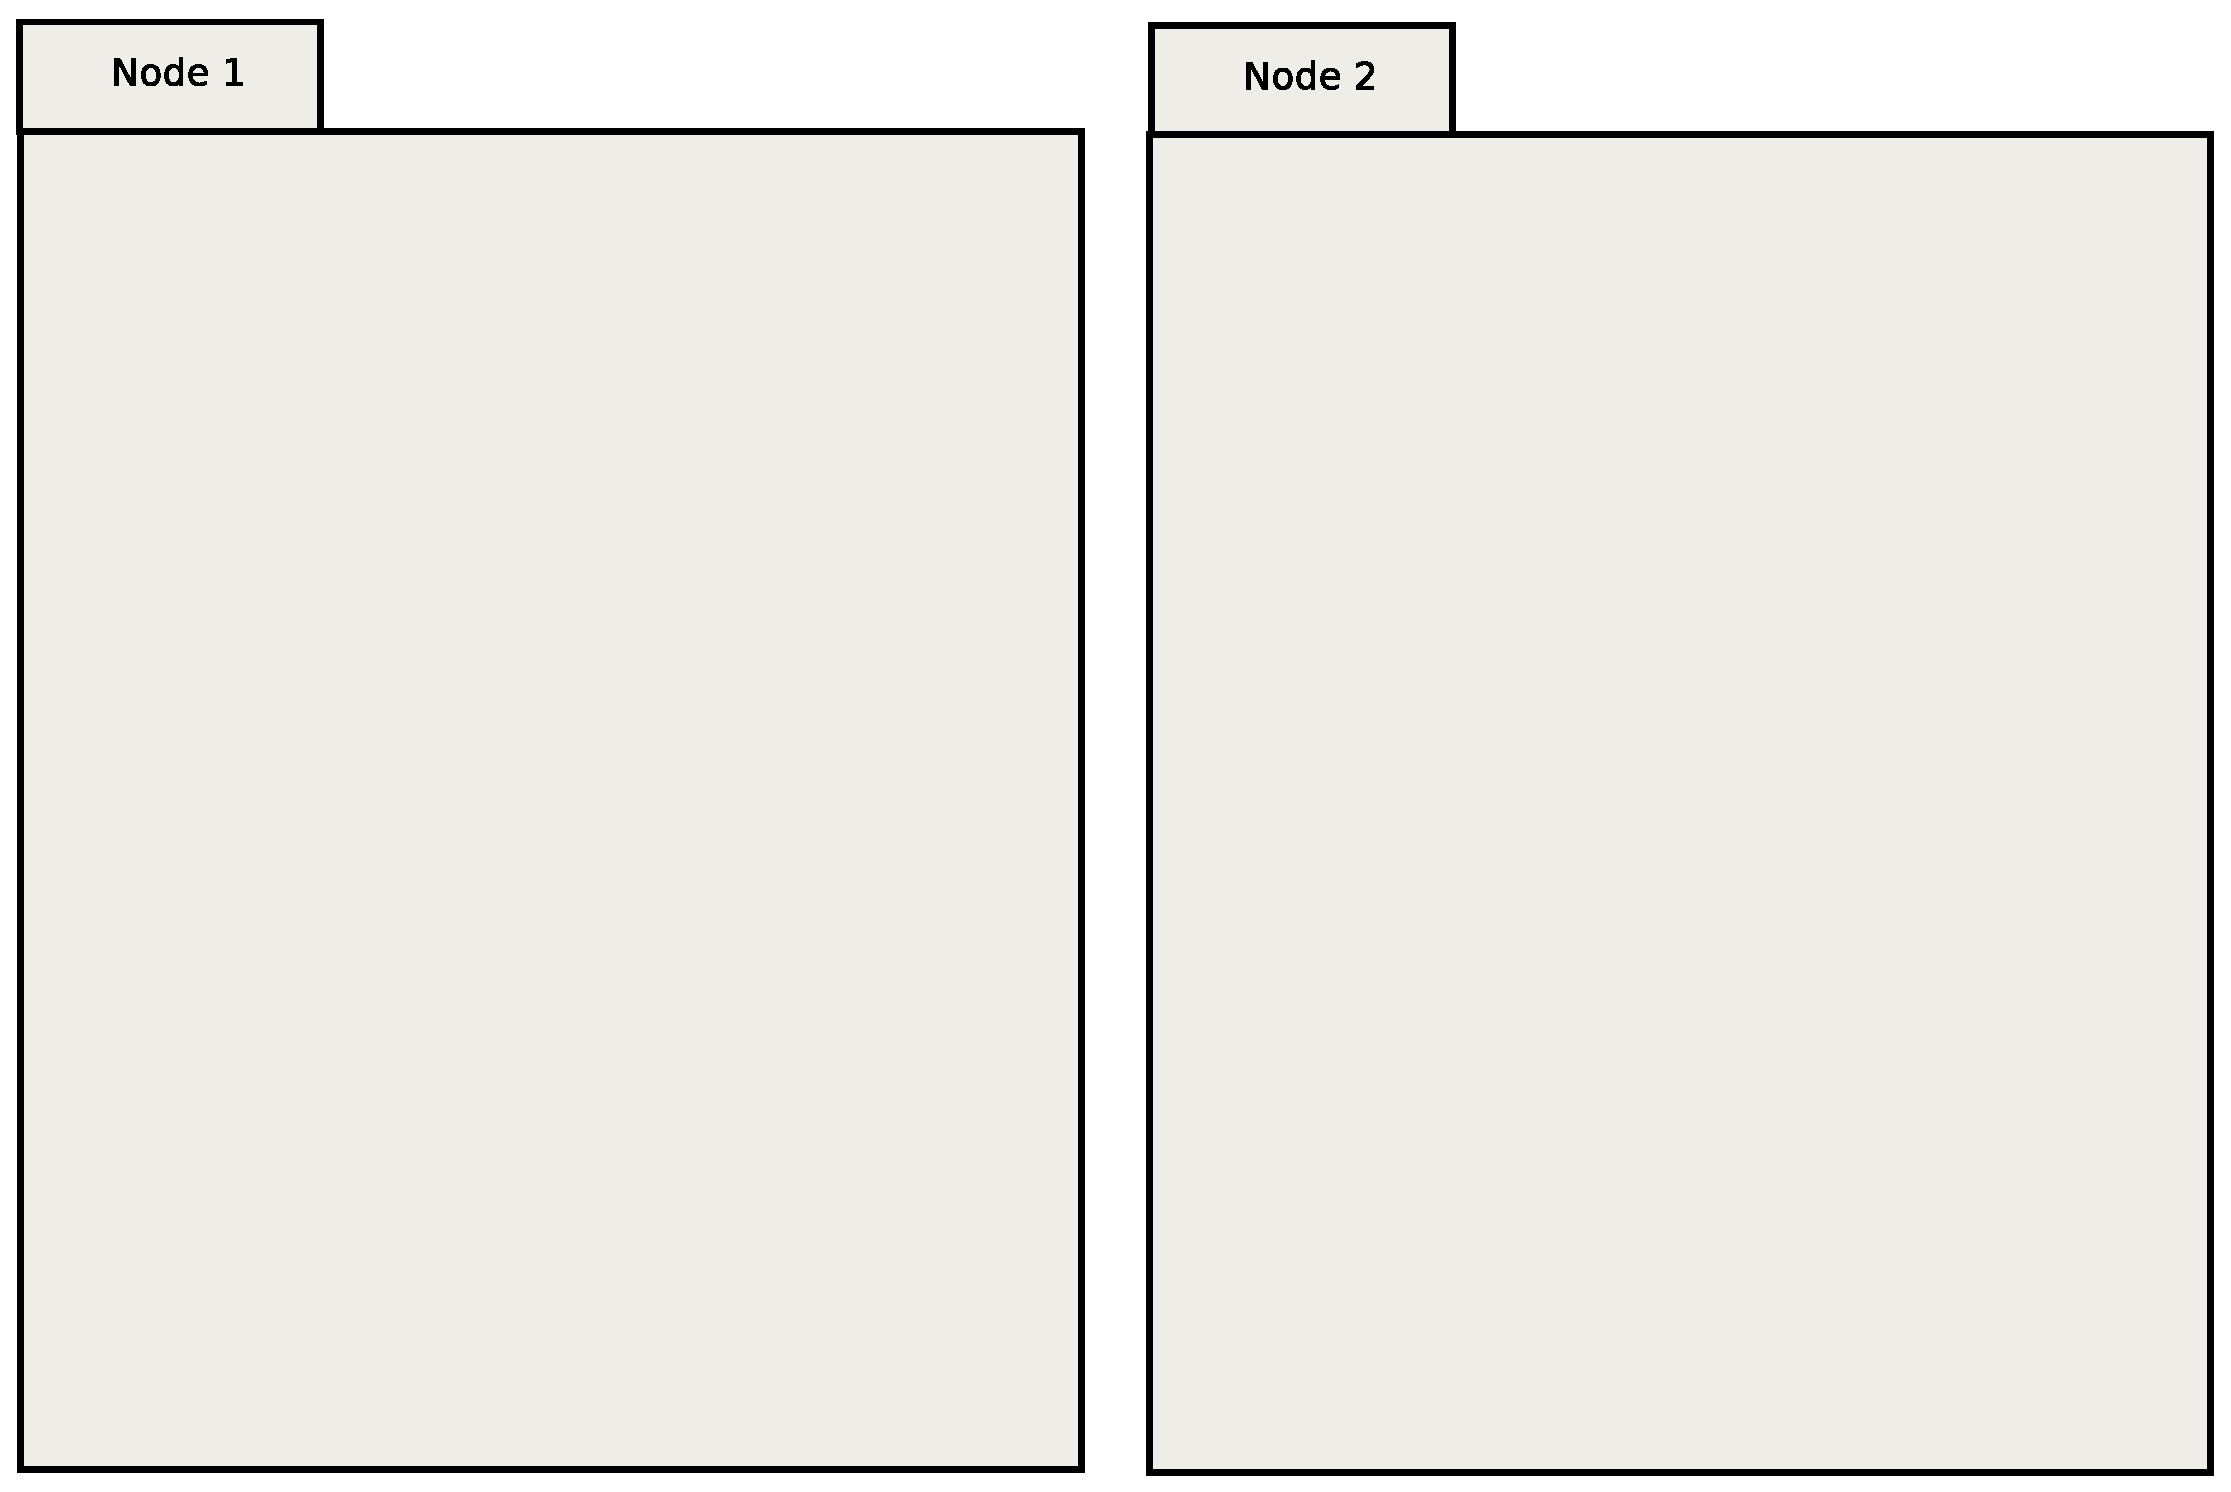
\includegraphics[width=\textwidth,height=0.85\textheight,keepaspectratio]{graphics/00-nodes.eps}
    \end{frame}

    \begin{frame}
        \frametitle{Pods}
        Pods (not Containers!) are the fundamental building blocks of a Kubernetes Application\pause
        \begin{itemize}
            \item A Pod is a group of one or more Containers that work closely together on a specific task.\pause
            \item Pods manage Volumes for their Containers.\pause
            \item Pods specify health check endpoints for their Containers.\pause
            \item Kubernetes software is deployed as Pods on the cluster!
        \end{itemize}
    \end{frame}

    \begin{frame}
        \frametitle{System Pods}
        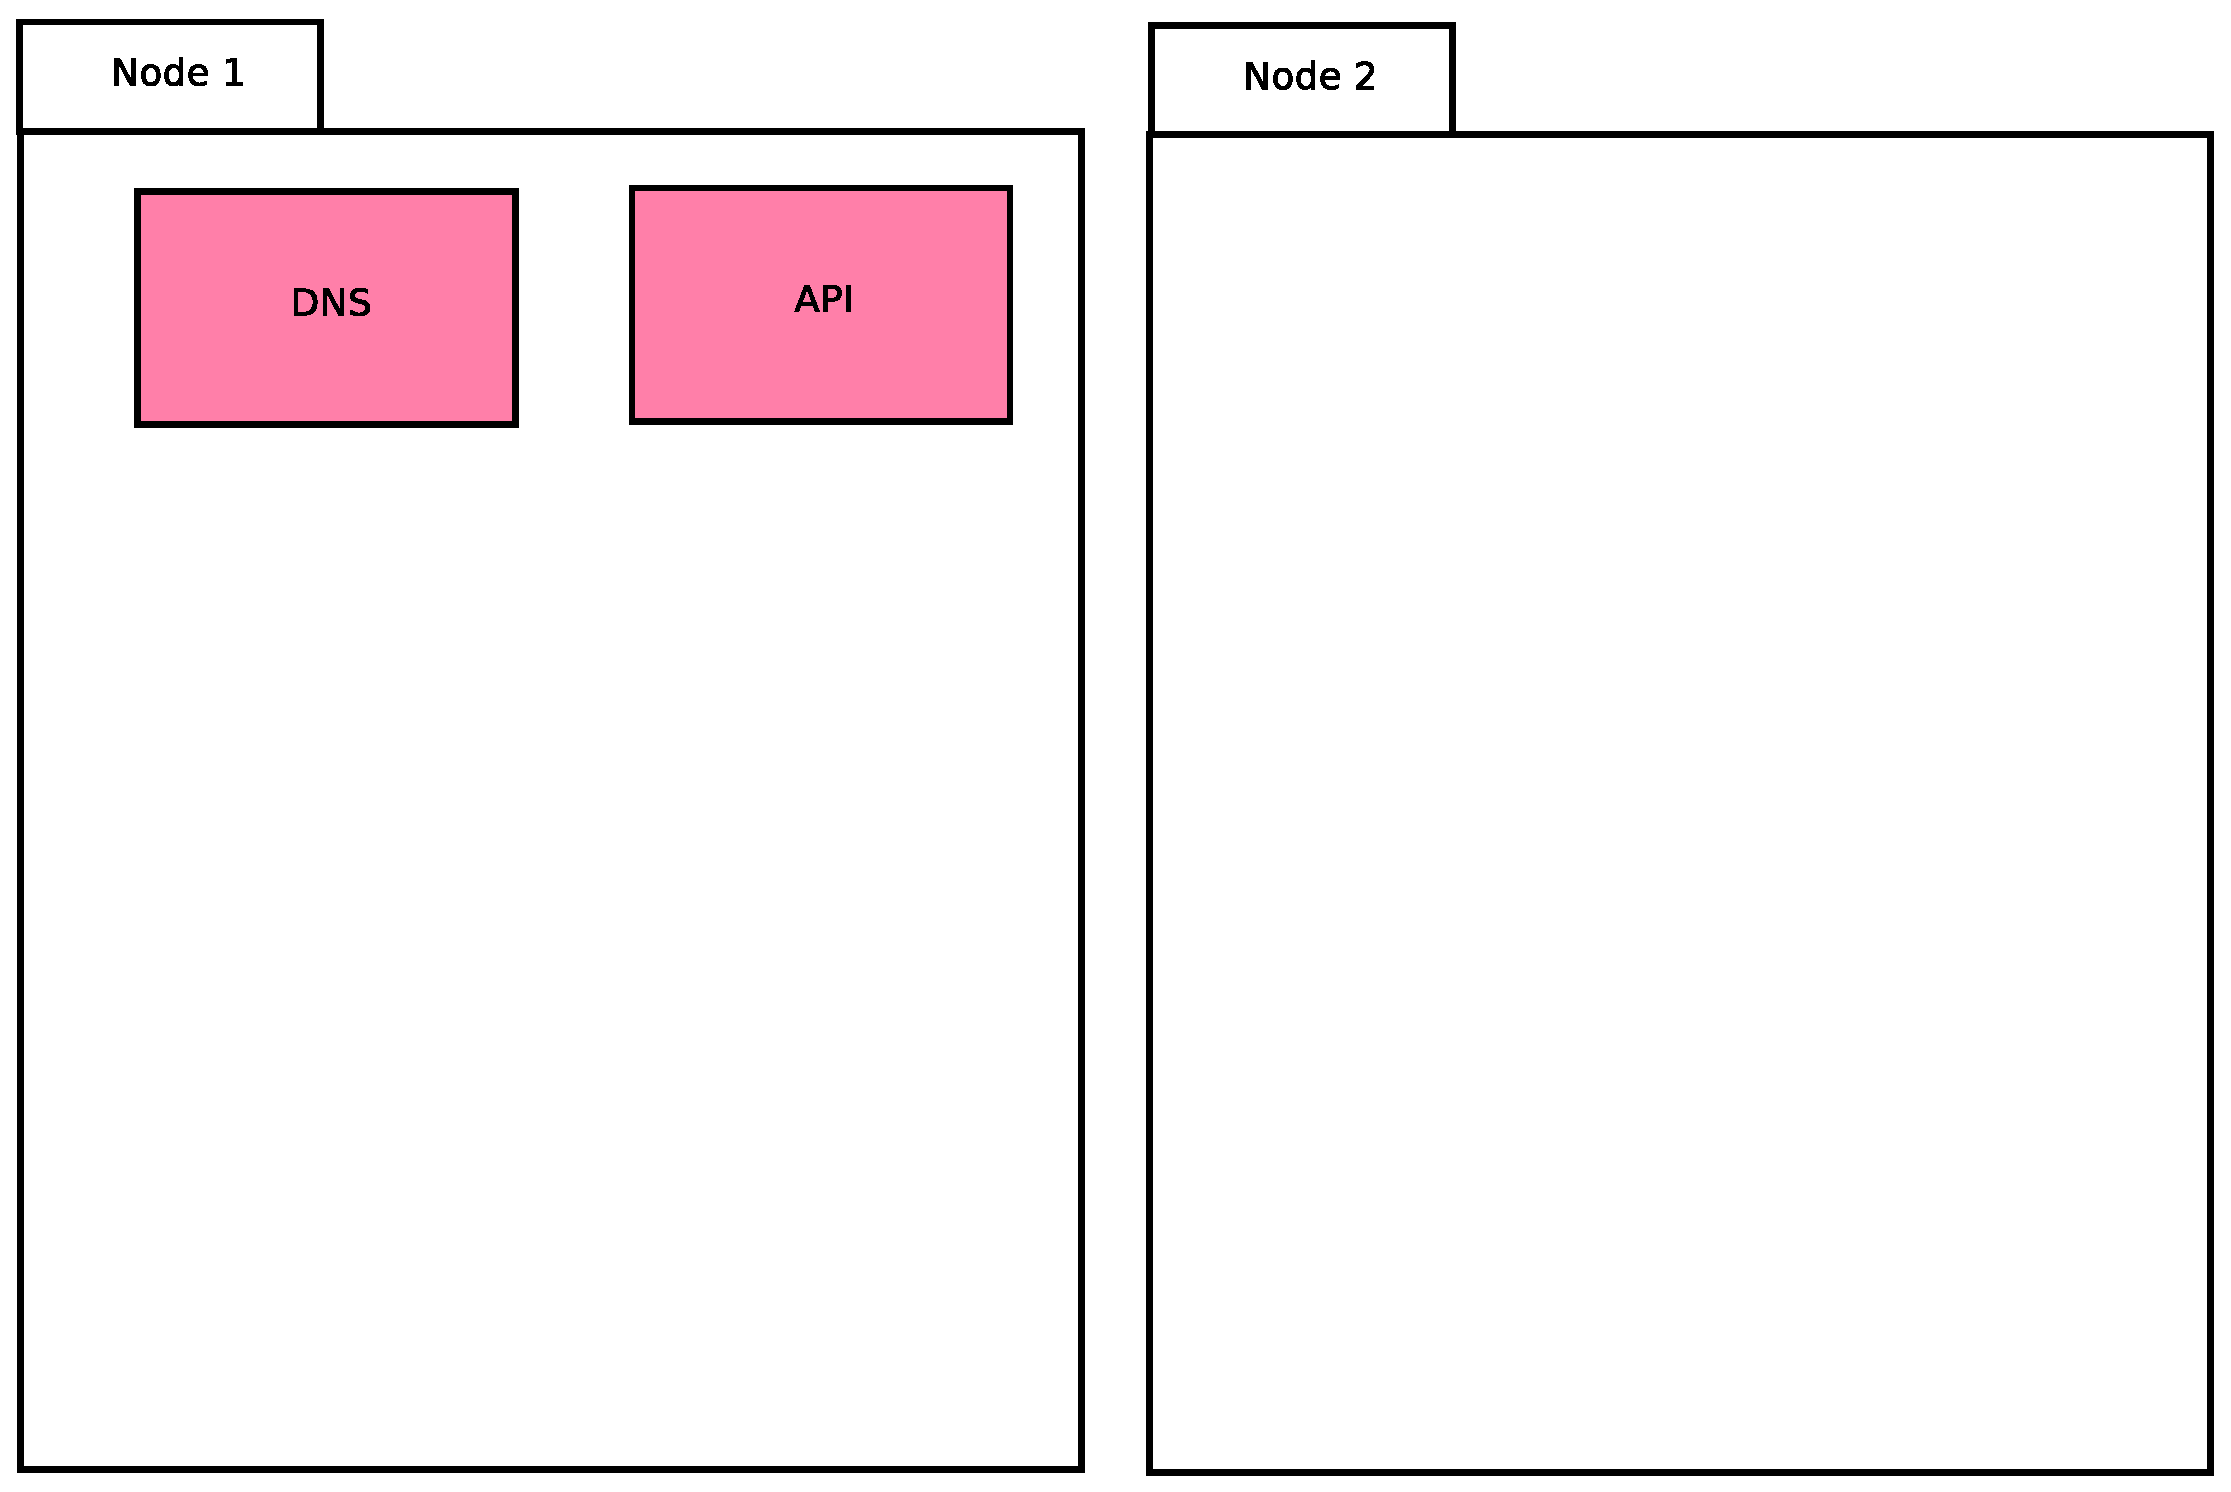
\includegraphics[width=\textwidth,height=0.85\textheight,keepaspectratio]{graphics/01-systemPods.eps}
    \end{frame}

    \begin{frame}
        \frametitle{The Sample Apps}
        I wrote two Applications that do nothing other than suggest a random Subreddit.\pause
        \begin{itemize}
            \item One is stateless:
            \begin{itemize}
                \item Selects at random from a list of 280 Subreddits.\pause
                \item The list never changes.\pause
                \item It doesn't need to store anything anywhere.\pause
            \end{itemize}
            \item One is stateful:
            \begin{itemize}
                \item Selects at random from a list of Subreddits.\pause
                \item \textbf{Removes} the selected Subreddit from the list.\pause
                \item Persists the list.\pause
                \item Uses the updated list to service the next request.
            \end{itemize}
        \end{itemize}
    \end{frame}

    \begin{frame}
        \frametitle{An Aside on Pods}
        \begin{itemize}
            \item Pods come and go.\pause
            \begin{itemize}
                \item Replaced if unresponsive.\pause
                \item Can be deleted on one Node and added on another (moved).\pause
                \item \textbf{You cannot prevent either of these things from happening.}\pause
            \end{itemize}
            \item By default, Volumes don't follow Pods.\pause
            \item By default, hostnames don't follow Pods.\pause
            \item Not a big deal for stateless Applications.\pause
            \item Definitely needs to be addressed for our stateful Application.
        \end{itemize}
    \end{frame}

    \begin{frame}
        \frametitle{Tool: docker\footnotemark}
        \begin{itemize}
            \item Our Applications need to be packaged as docker Containers.
            \item We need publish these Containers to minikube's docker server.
        \end{itemize}
        \footnotetext[1]{\href{https://www.docker.com/get-started}{https://www.docker.com/get-started}}
    \end{frame}

    \begin{frame}
        \frametitle{Stateless Application Pods}
        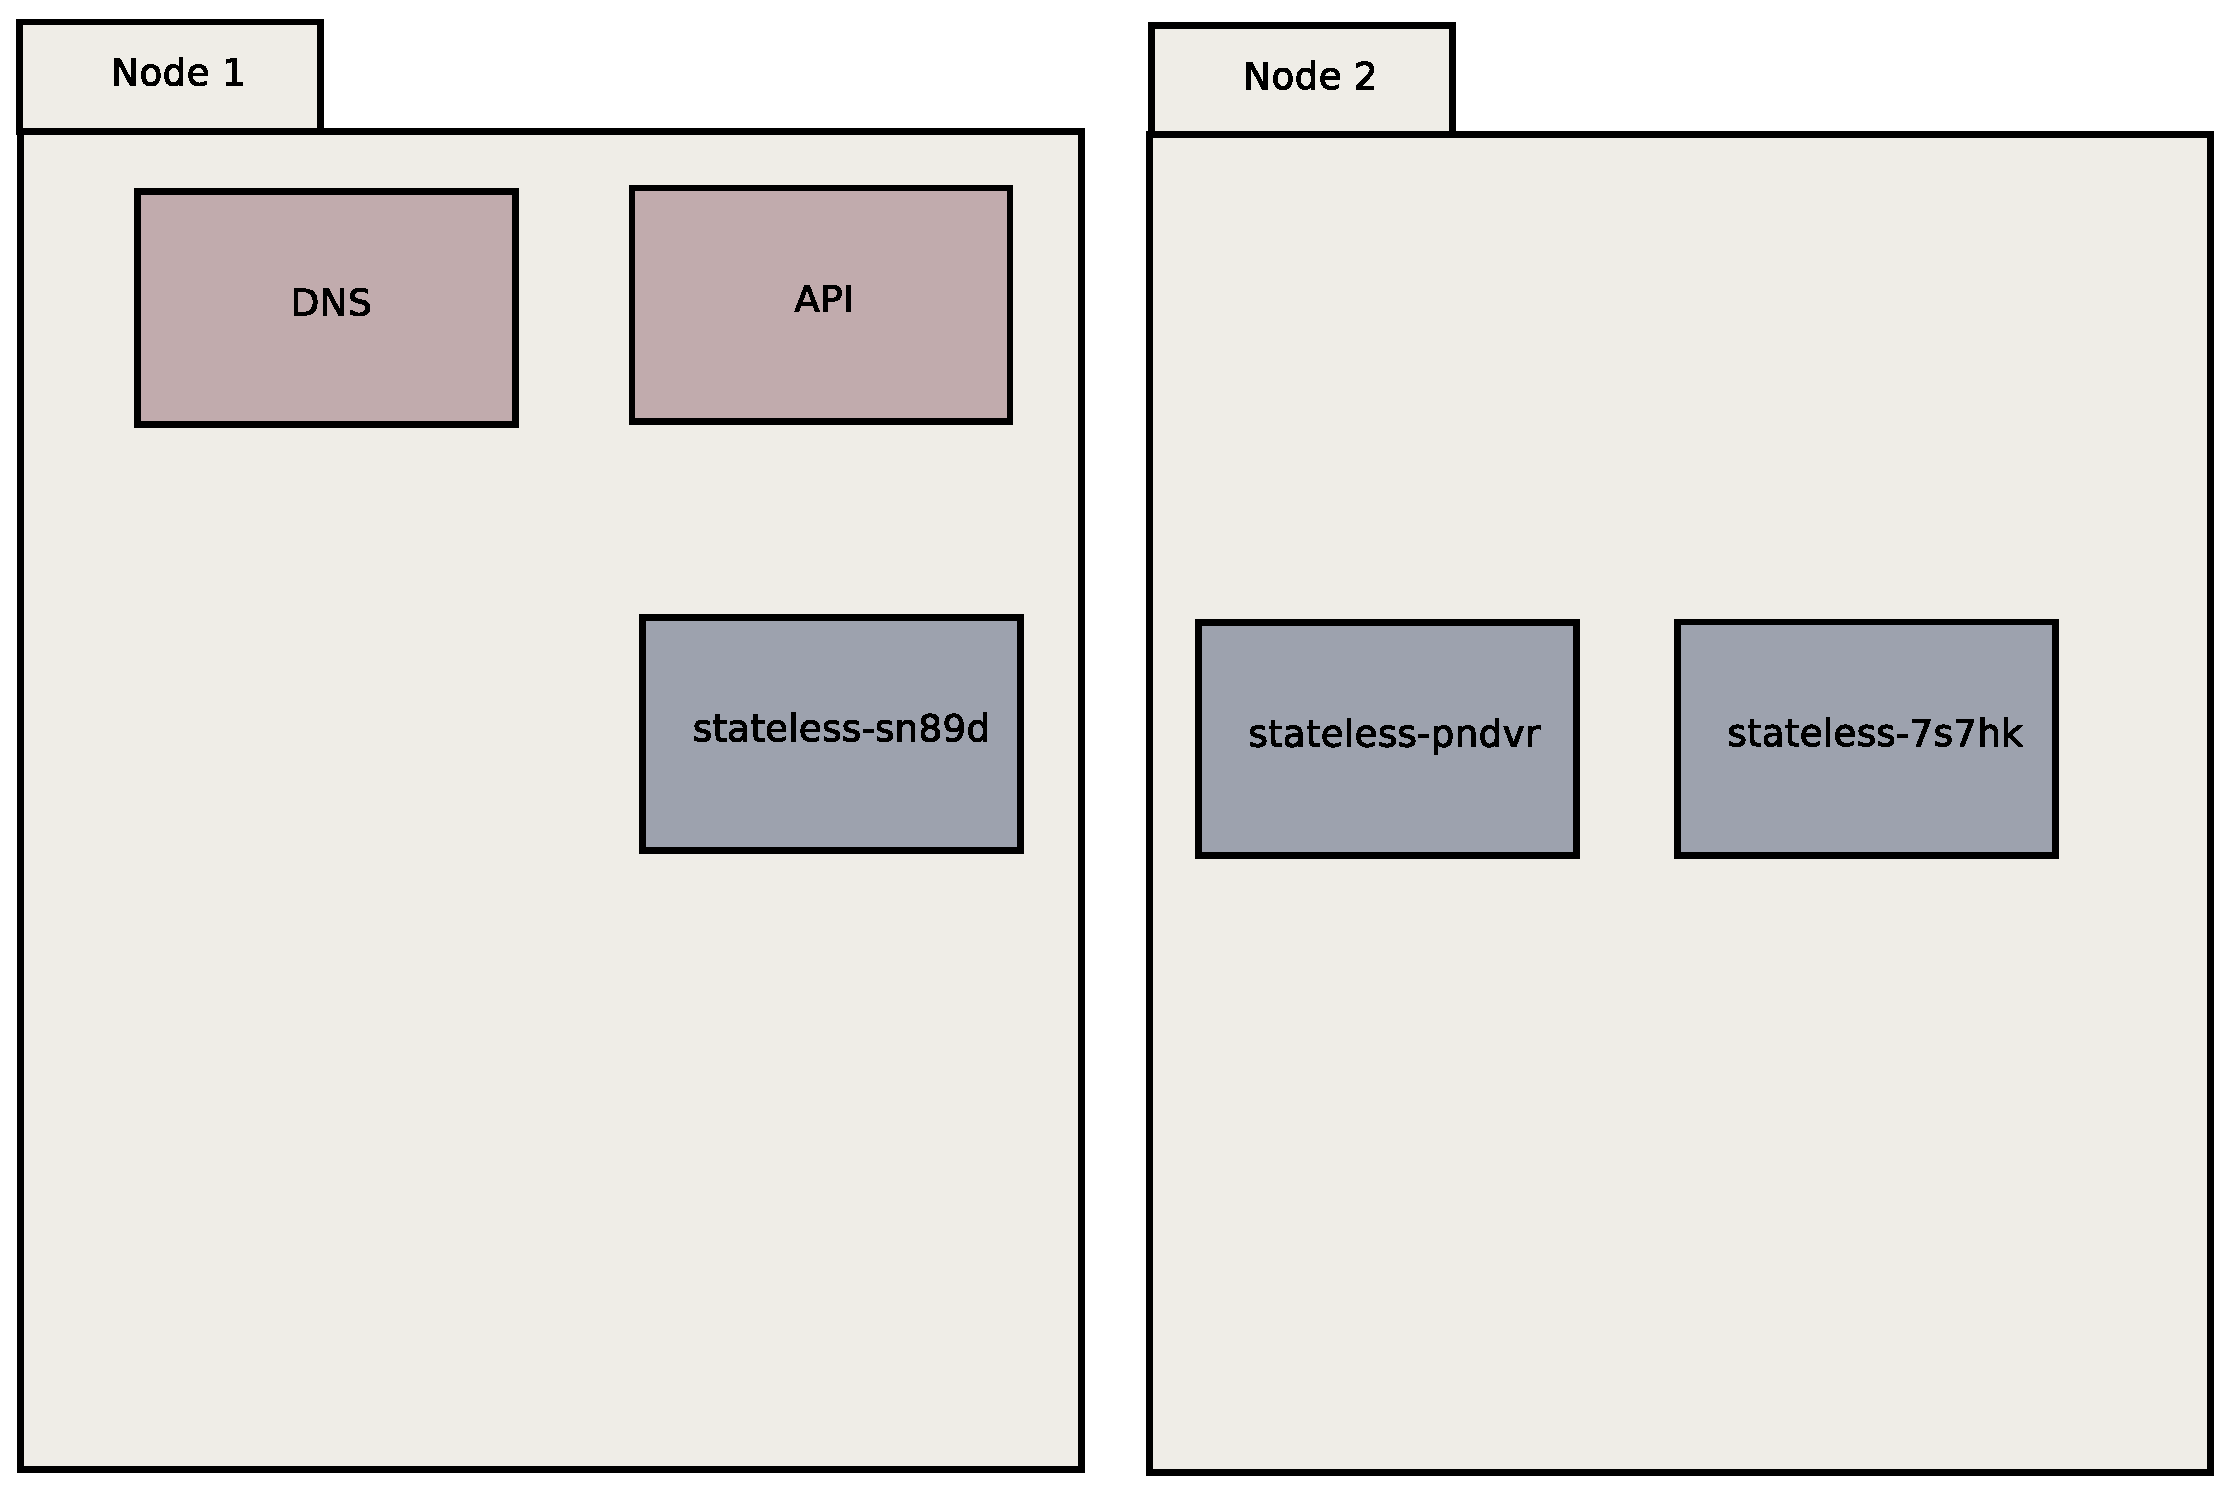
\includegraphics[width=\textwidth,height=0.85\textheight,keepaspectratio]{graphics/02-statelessAppPods.eps}
    \end{frame}

    \begin{frame}
        \frametitle{Stateful Application Pods}
        \includegraphics[width=\textwidth,height=0.85\textheight,keepaspectratio]{graphics/03-statefulAppPods.eps}
    \end{frame}

    \begin{frame}
        \frametitle{Controllers}
        \begin{itemize}
            \item Don't create Pods directly.
            \item Instead, create a Controller that manages the Pods for you.
        \end{itemize}
    \end{frame}

    \begin{frame}
        \frametitle{Controllers: ReplicaSets}
        \begin{itemize}
            \item State how many Pods you want.\pause
            \item Pods are treated as if they were stateless.\pause
            \item From Application's point of view, Pods in a ReplicaSet are indistinguishable.
        \end{itemize}
    \end{frame}

    \begin{frame}
        \frametitle{Controllers: Deployments}
        \begin{itemize}
            \item ReplicaSets with more features.\pause
            \item I'm not going to use those features.\pause
            \item But I use Deployments because helm produces them for skeleton helm projects.
        \end{itemize}
    \end{frame}

    \begin{frame}
        \frametitle{Controllers: StatefulSets}
        StatefulSets manage Pods that are required to have state, namely:\pause
        \begin{itemize}
            \item Pods in a StatefulSet each have a persistent network identity.\pause
            \item Pods in a StatefulSet each have persistent storage.\pause
            \item ``Persistent" here means they ``follow" Pods.\pause
            \item Good news for our stateful Application.
        \end{itemize}
    \end{frame}

    \begin{frame}
        \frametitle{Tool: kubectl\footnotemark}
        kubectl can:
        \begin{itemize}
            \item Update components in our cluster.\pause
            \item Inspect components in our cluster.\pause
            \item Create components in our cluster, but we'll use another tool for that...
        \end{itemize}
        \footnotetext[1]{\href{https://kubernetes.io/docs/tasks/tools/install-kubectl}{https://kubernetes.io/docs/tasks/tools/install-kubectl}}
    \end{frame}

    \begin{frame}
        \frametitle{Tool: helm\footnotemark}
        \begin{itemize}
            \item Tool for packaging and deploying Kubernetes Applications.
            \item We'll use helm (instead of kubectl) to create our Kubernetes components.
        \end{itemize}
        \footnotetext[1]{\href{https://helm.sh}{https://helm.sh}}
    \end{frame}

    \begin{frame}
        \frametitle{Deployment}
        \includegraphics[width=\textwidth,height=0.85\textheight,keepaspectratio]{graphics/04-deployment.eps}
    \end{frame}

    \begin{frame}
        \frametitle{StatefulSet}
        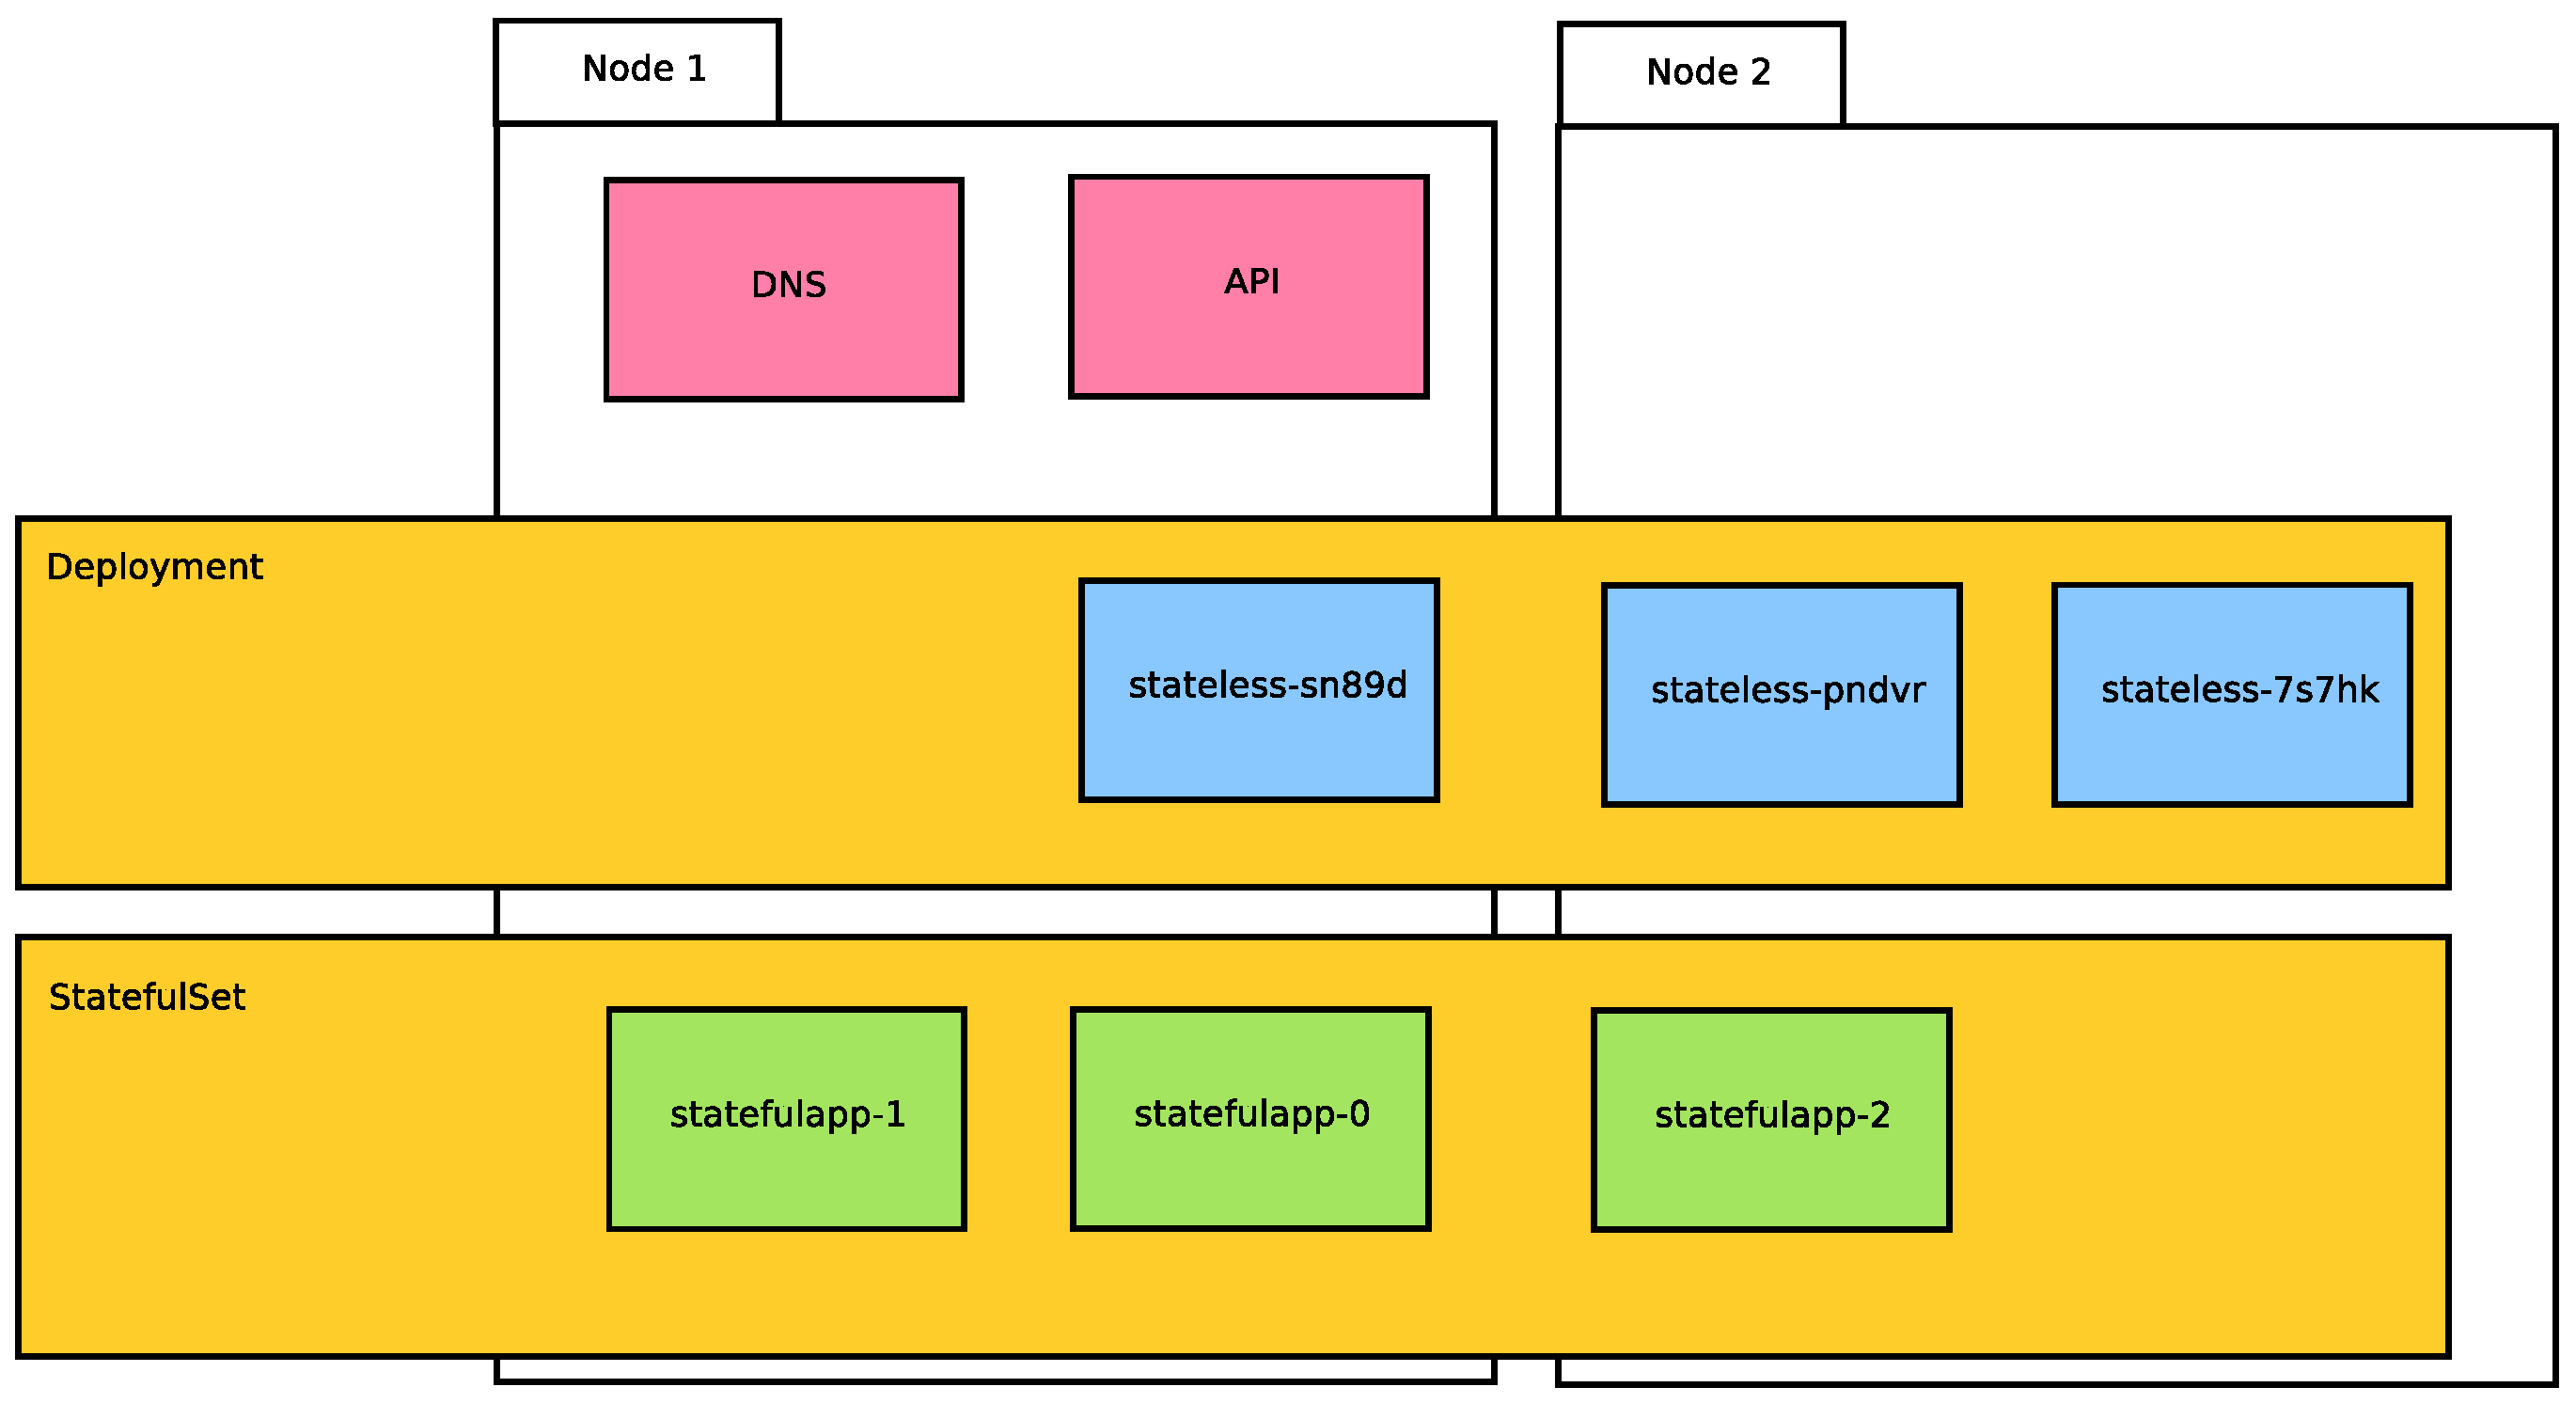
\includegraphics[width=\textwidth,height=0.85\textheight,keepaspectratio]{graphics/05-statefulSet.eps}
    \end{frame}

    \begin{frame}
        \frametitle{StatefulSet: Persistent Storage}
        \begin{itemize}
            \item StatefulSet Pods can have PersistentVolumeClaims (PVCs).\pause
            \item PVCs are used to request PersistentVolumes.\pause
            \item PersistentVolumes are Volumes that survive Pods being moved or replaced.
        \end{itemize}
    \end{frame}

    \begin{frame}
        \frametitle{StatefulSet: Persistent Storage}
        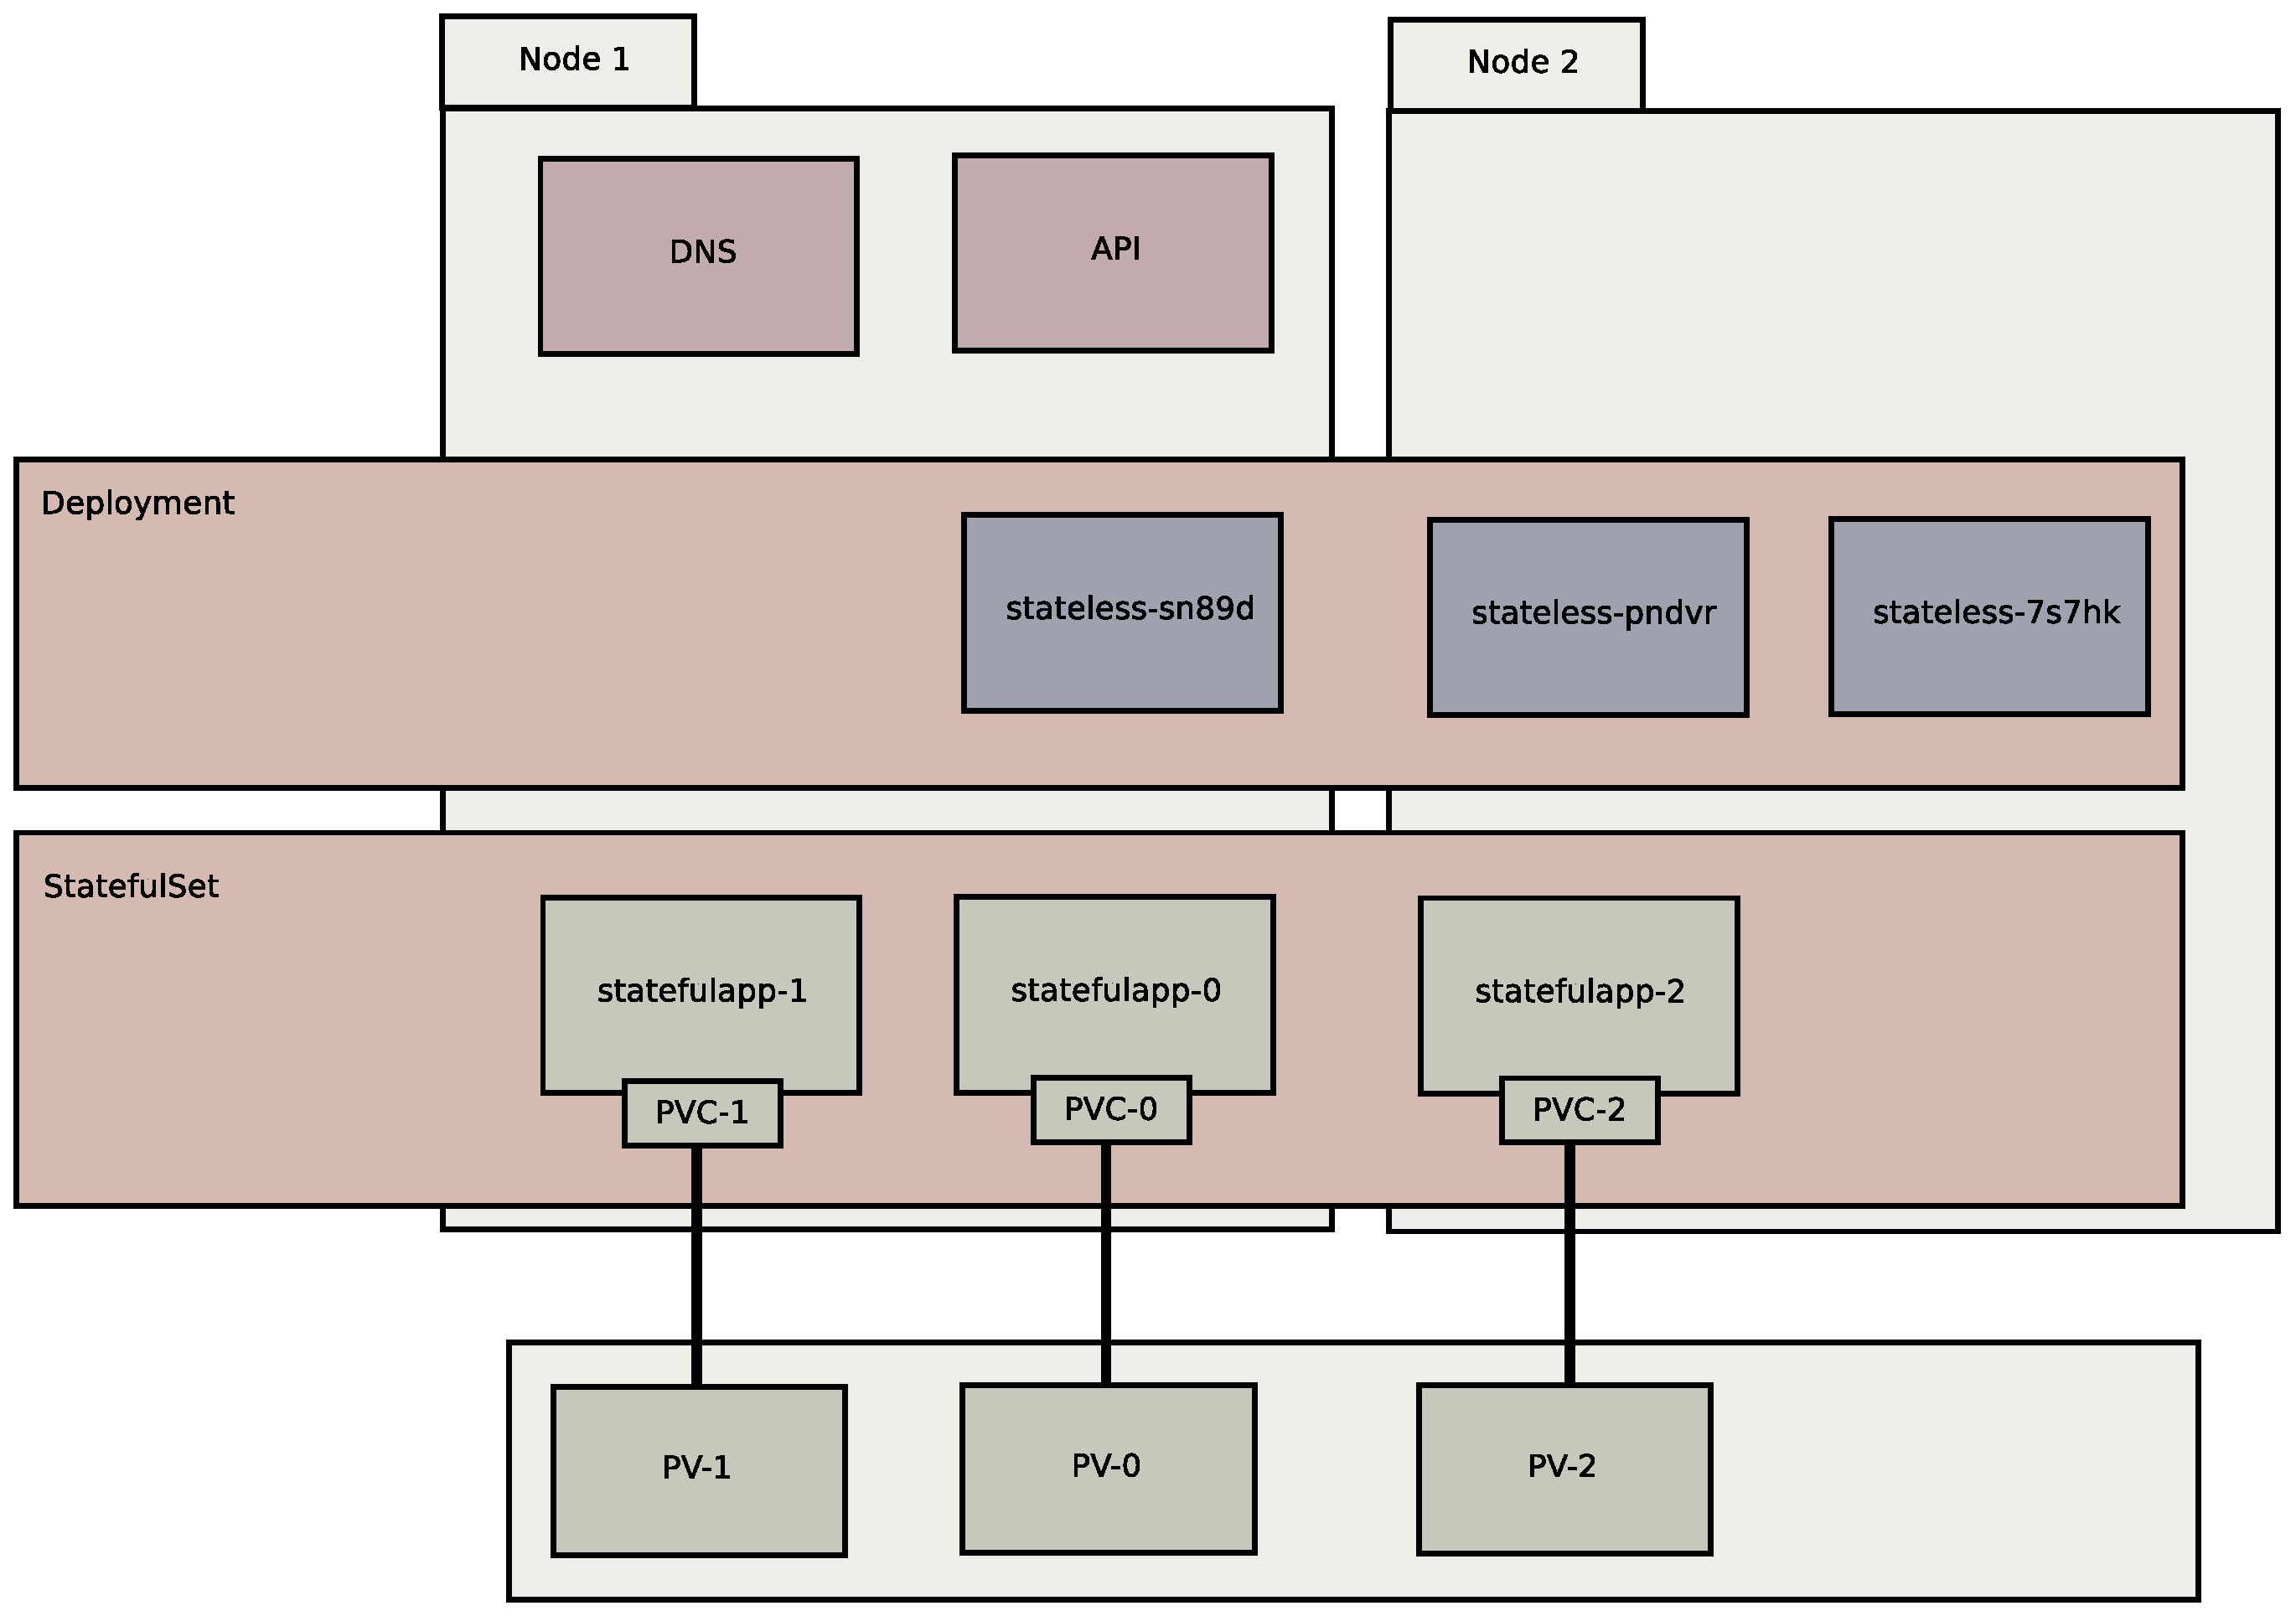
\includegraphics[width=\textwidth,height=0.85\textheight,keepaspectratio]{graphics/06-persistence.eps}
    \end{frame}

    \begin{frame}
        \frametitle{StatefulSet: Headless Service}
        StatefulSets require a Headless Service
        \begin{itemize}
            \item It's used by the Kubernetes DNS Pod.\pause
            \item It allows Pods to keep their hostname by keeping track of their IP address (even when it changes).
        \end{itemize}
    \end{frame}

    \begin{frame}
        \frametitle{StatefulSet: Headless Service}
        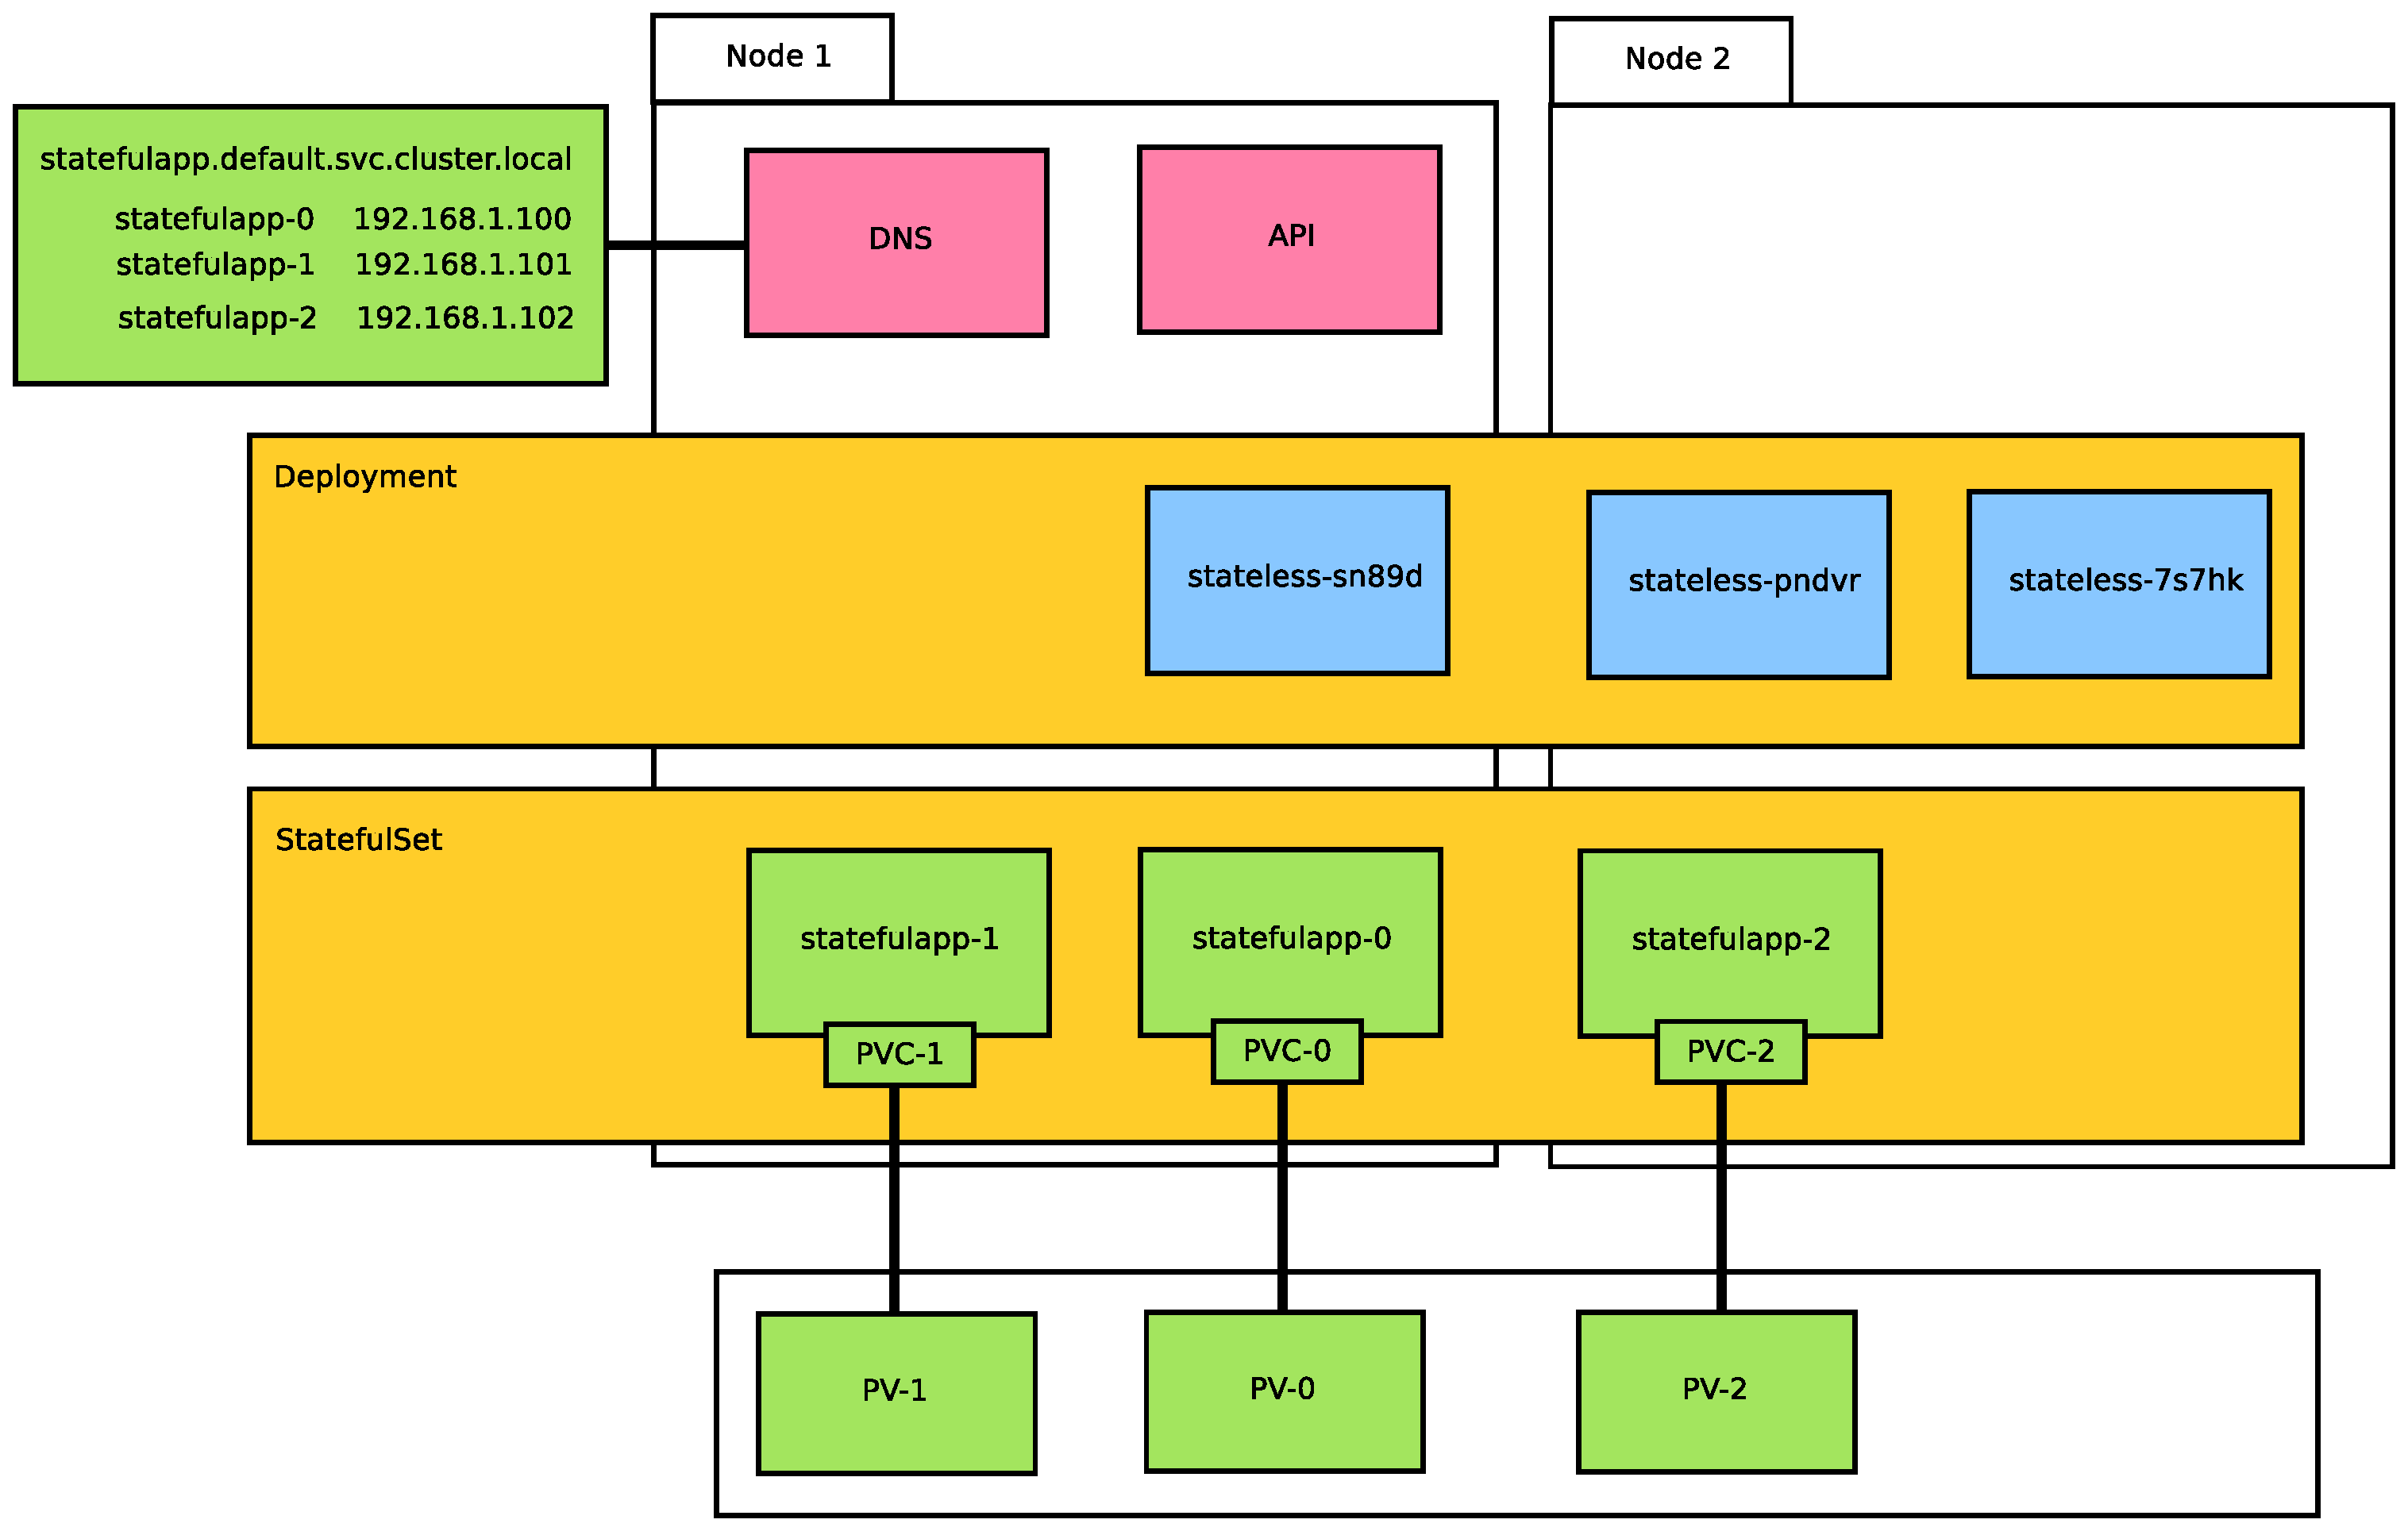
\includegraphics[width=\textwidth,height=0.85\textheight,keepaspectratio]{graphics/07-persistentIdentity.eps}
    \end{frame}

    \begin{frame}
        \frametitle{Load Balancers}
        \begin{itemize}
            \item Load Balancers have an internal cluster IP address.\pause
            \item They can also have an external IP address.\pause
            \item They distribute requests sent to either IP address to all Pods targeted by their ``selector".
        \end{itemize}
    \end{frame}

    \begin{frame}
        \frametitle{Load Balancers}
        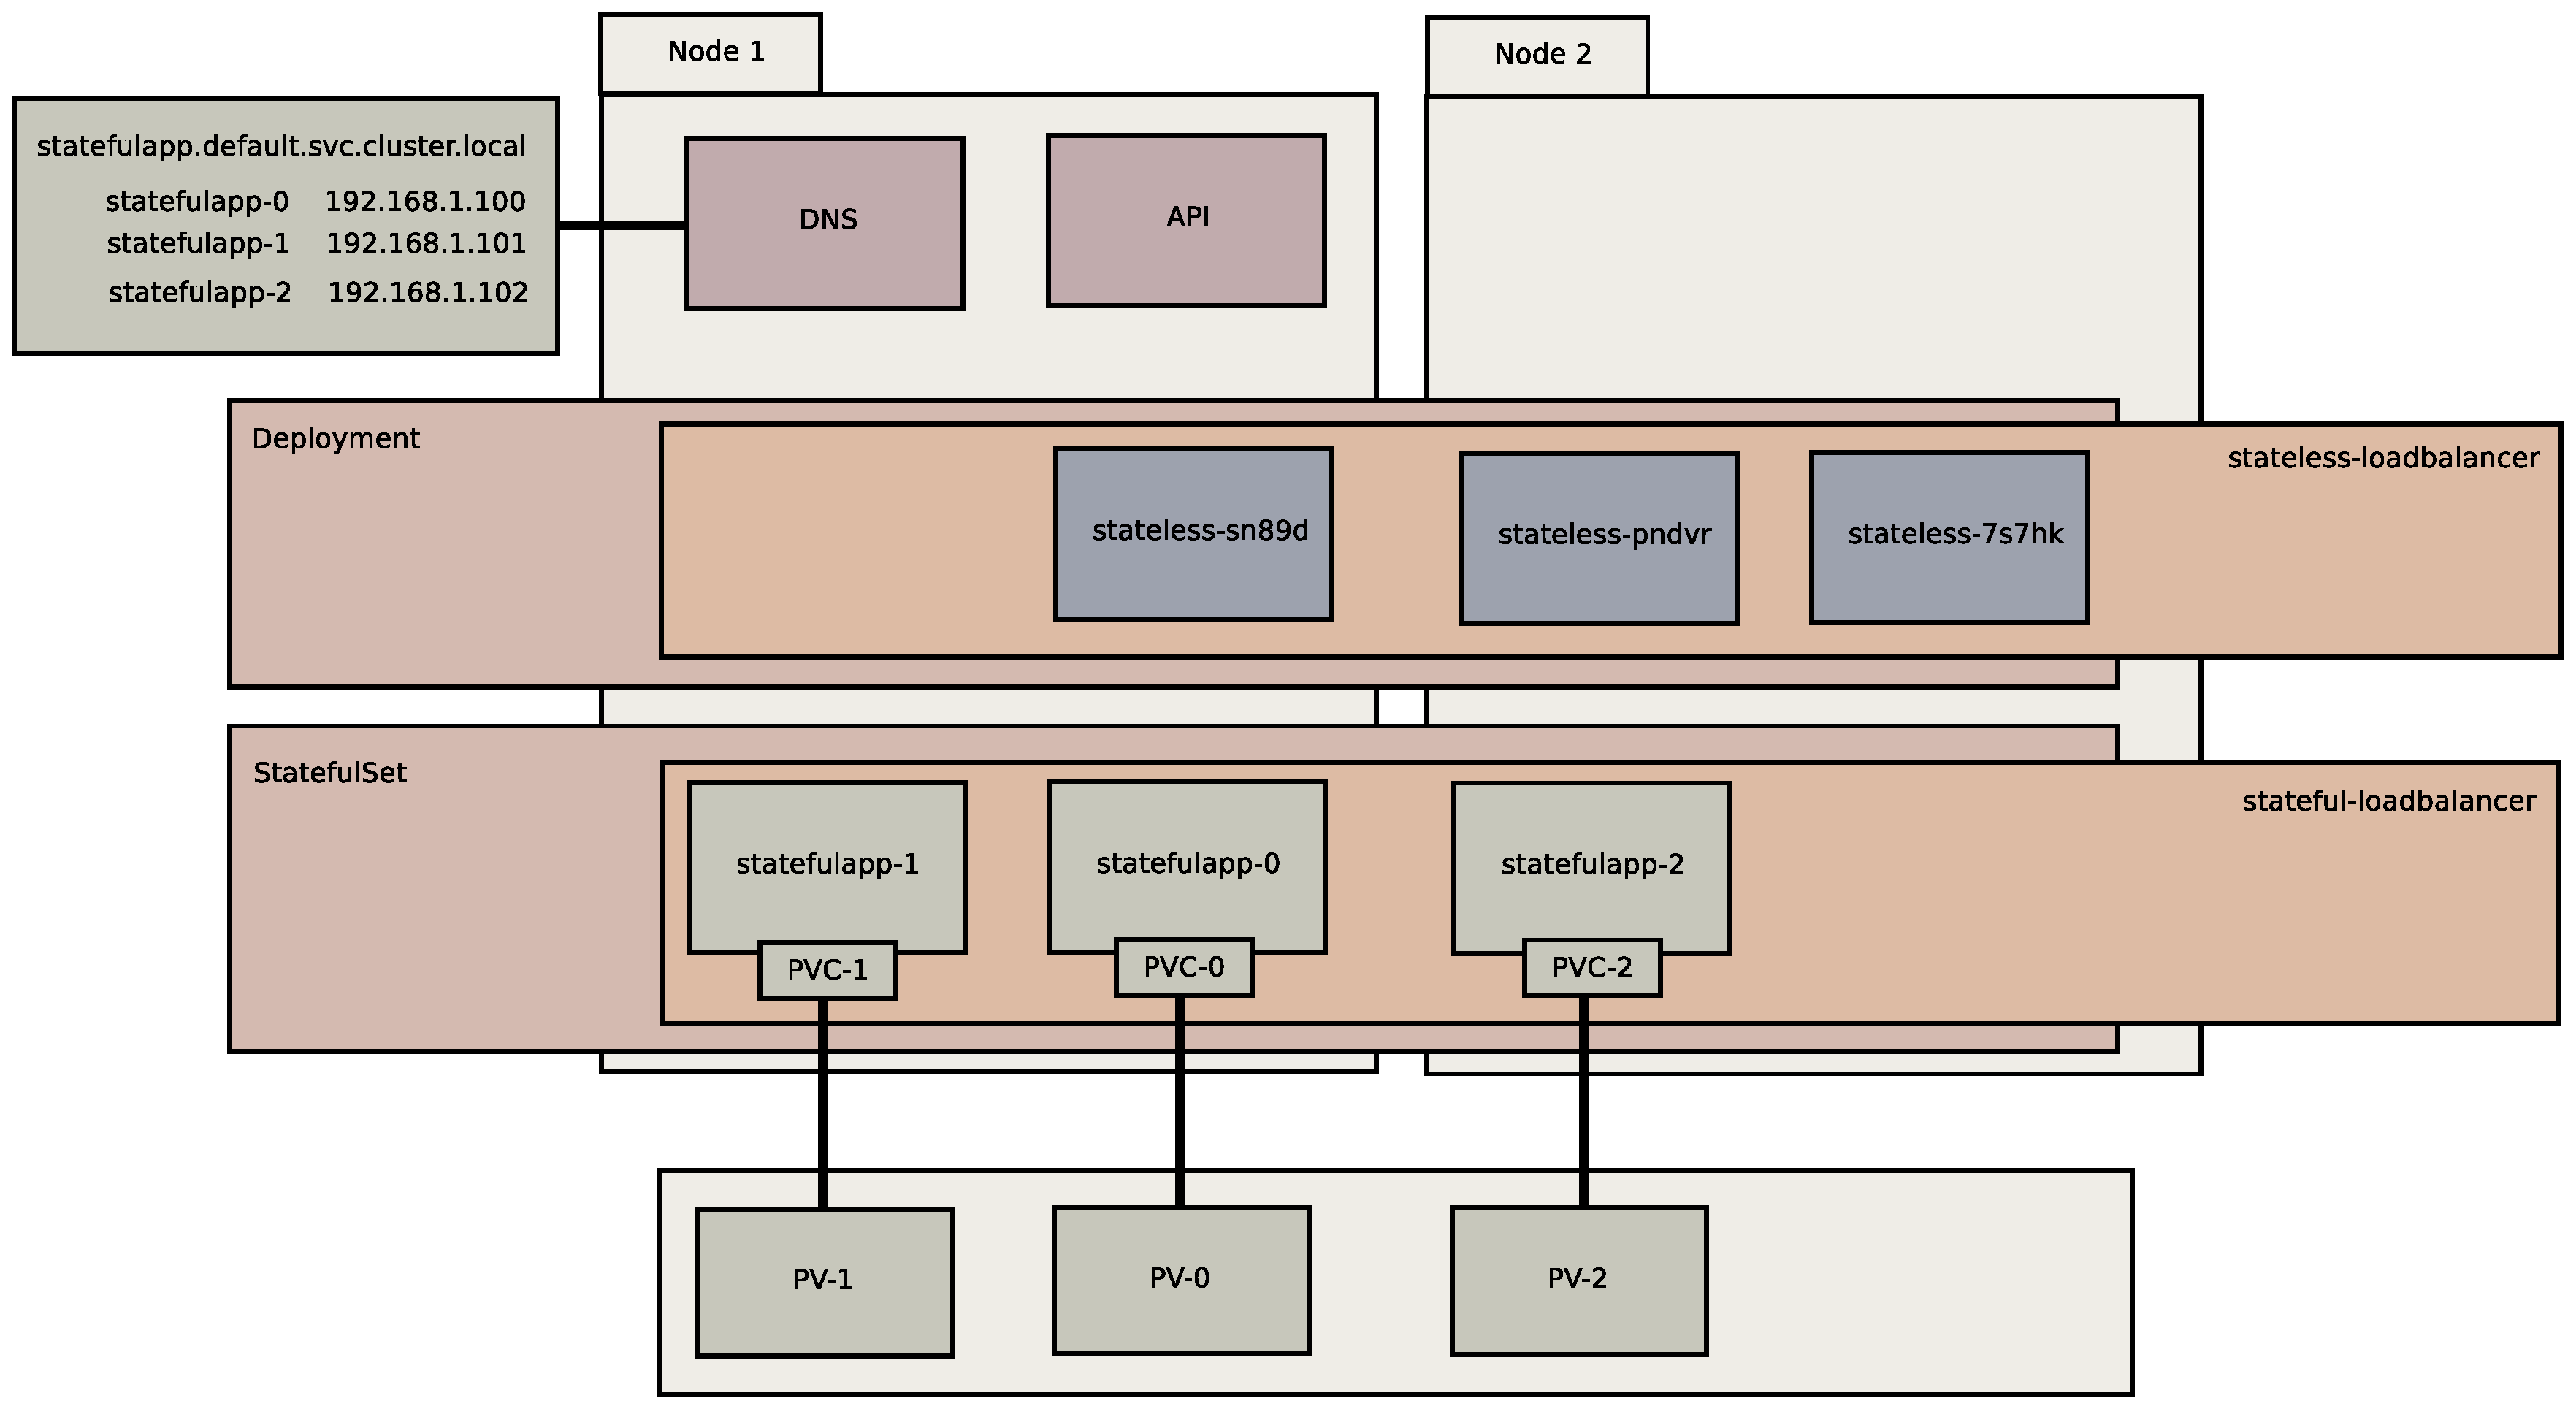
\includegraphics[width=\textwidth,height=0.85\textheight,keepaspectratio]{graphics/08-loadBalancer.eps}
    \end{frame}

    \begin{frame}
        \frametitle{Demo}
        \begin{center}
            \Huge So, let's see this in action!
        \end{center}
    \end{frame}

    \begin{frame}
        \frametitle{Overview}
        First, let's talk about the steps we're going to take:
        \begin{itemize}
            \item Start our Kubernetes environment (minikube).\pause
            \item Configure our docker cli to talk to minikube's docker host.\pause
            \item Build our two sample Applications, package them as docker Containers, and push the images.\pause
            \item Run helm to deploy our Kubernetes components.\pause
            \item Proxy local ports to connect to our load balancing services.
        \end{itemize}
    \end{frame}

    \begin{frame}
        \frametitle{Demo: Simplified Architecture}
        \includegraphics[width=\textwidth,height=0.85\textheight,keepaspectratio]{graphics/simplifiedModel-00.eps}
    \end{frame}

    \begin{frame}
        \begin{center}
            \Huge Is there enough time to go deeper?\\
            If so, let's dig into some code.
        \end{center}
    \end{frame}

    \begin{frame}
        \frametitle{Other Resources}
        Peripheral tools I used -- some of which warrant their own presentation
        \begin{itemize}
            \item \LaTeX: \href{https://www.latex-project.org}{https://www.latex-project.org}
            \item Beamer: \href{https://ctan.org/pkg/beamer}{https://ctan.org/pkg/beamer}
            \item Kotlin: \href{https://kotlinlang.org}{https://kotlinlang.org}
            \item Spring Boot: \href{https://spring.io/projects/spring-boot}{https://spring.io/projects/spring-boot}
            \item Gradle: \href{https://gradle.org}{https://gradle.org}
            \item Dia: \href{http://dia-installer.de}{http://dia-installer.de}
        \end{itemize}
        \smallskip
        Where I got my Subreddit data
        \begin{itemize}
            \item Bulk Reddit data: \href{http://files.pushshift.io/reddit/subreddits}{http://files.pushshift.io/reddit/subreddits}
        \end{itemize}
        Finally, \textbf{\textit{this}} demo
        \begin{itemize}
            \item \href{https://github.com/emacdona/k8sdemo}{https://github.com/emacdona/k8sdemo}
        \end{itemize}
    \end{frame}

    \begin{frame}
        \frametitle{A Note on Capitalization}
        I agonized over which words to capitalize.
        \begin{itemize}
            \item{I capitalized important concepts in the Kubernetes domain:}
            \begin{itemize}
                \item{Any Kubernetes component: Deployment, Pod, ReplicaSet, StatefulSet, ...}
                \item{Application, Container, Kubernetes, Node, Volume}
            \end{itemize}

            \item{But some didn't quite make the cut:}
            \begin{itemize}
                \item{cluster, component}
            \end{itemize}

            \item{I could not bring myself to capitalize things that I type at the command prompt:}
            \begin{itemize}
                \item{docker, helm, kubectl, minikube}
            \end{itemize}
        \end{itemize}
    \end{frame}

    \begin{frame}
        \begin{center}
            \Huge Questions?
        \end{center}
    \end{frame}

\end{document}
